\RequirePackage{plautopatch}
\documentclass[platex,dvipdfmx,10pt,a4j]{jarticle}
\usepackage{setspace}
\usepackage{url}
\usepackage[dvipdfmx]{graphicx}
\usepackage{float}
\usepackage{fancyhdr}
\usepackage[title]{appendix}
\usepackage{amsmath}
\usepackage{multirow}
\usepackage{bm}
\usepackage{amssymb}

\renewcommand{\figurename}{Fig}
\renewcommand{\tablename}{Table}
\renewcommand{\refname}{参考文献}

\pagestyle{fancy}
\rhead{}
\lhead{\rightmark}
\cfoot{\thepage}
\rfoot{}
\renewcommand{\footrulewidth}{0.4pt}

\begin{document}
\begin{center}

    \thispagestyle{empty}

    \vspace*{10pt}

    \begin{spacing}{2}
        {\Huge \underline{機能デザイン研究I\hspace{-.1em}I}}
    \end{spacing}

    \begin{spacing}{2}
        \vspace{\baselineskip}
    \end{spacing}

    {\LARGE 令和2年2月7日提出}

    \begin{spacing}{2}
        \vspace{\baselineskip}
    \end{spacing}

    \vskip 5.8zh
    \[ \left. \begin{array}{ll}
            \mbox{{\LARGE 杉山 和靖}} & \mbox{{\LARGE 教授}} \\
            \mbox{{\LARGE 渡村 友昭}} & \mbox{{\LARGE 助教}}
        \end{array} \right\} \mbox{{\LARGE 指導}}
    \] \par
    \vskip 5.3zh

    \begin{spacing}{2}
        \vspace{\baselineskip}
    \end{spacing}

    \begin{spacing}{1.2}
        {\LARGE 大阪大学大学院 基礎工学研究科 機能創成専攻}
    \end{spacing}
    \begin{spacing}{1.2}
        {\LARGE 機能デザイン領域 推進工学講座}
    \end{spacing}
    \begin{spacing}{1.2}
        {\LARGE 29B20038}
    \end{spacing}
    \begin{spacing}{2}
        \vspace{\baselineskip}
    \end{spacing}
    \begin{spacing}{1.8}
        {\LARGE 丹羽 英人}
    \end{spacing}
\end{center}

\newpage
\tableofcontents
\newpage
\section{緒言}

\subsection{研究背景}

一般的に,流体はせん断応力がせん断速度に比例するNewton流体と,せん断応力がせん断速度が非線形となる非Newton流体に分類することができる.様々な流体のせん断速度とせん断応力の関係をFig\ref{fig:1-fluid-curve}(a)に示す\cite{ref:1}.Newton流体はせん断速度とせん断応力が比例関係にある流体である.一方でそれ以外の流体は非Newton流体と呼ばれている.非Newton流体には Shear thinning 流体(Pseudoplastic), Shear thickening 流体(Dilatant fluid), Bingham plastic 流体, Viscoplastic 流体, Viscoelastic 流体が挙げられる.非Newton流体のうち,Bingham plastic 流体, Viscoplastic 流体は外力によるせん断応力がある値を超えないとせん断速度が発生しない流体である.これらの例として,バターや冷却途中の溶岩などが挙げられる\cite{mendes2004viscosity,balmforth2000visco}.一方で,Shear-thinning 流体, Shear-thinning 流体はせん断応力が少しでも加わると,せん断速度が発生し流体的挙動を示す.Shear-thinning 流体の例として,マヨネーズや血液,泥,ポリマーなどが挙げられる\cite{liu2007rheological,bodnar2011shear,hu2017shear,ryder2006shear}.Shear-thickening 流体の例として,水溶き片栗粉や液体ボディアーマー,ブレーキパッドなどが挙げられる\cite{crawford2013shear,haris2017effectiveness,zarei2020application}.また,Viscoelastic 流体は粘性だけでなく弾性的挙動を示す流体である.この例として流動ゴムや高分子融体が挙げられる\cite{stieger2021influence,boger1987viscoelastic}.

非Newton流体の粘度を表すモデルには,Power-law model (Ostwald-De Waele model)\cite{Ostwald1929}, Cross model\cite{cross1965rheology}, Carreau model\cite{carreau1972rheological}, Carreau-Yasuda model\cite{yasuda1979investigation}やHerschel-Bulkley model\cite{briscoe1994properties,de1998fresh}などがある\cite{ref:1}.Power-law model はせん断速度の限られた範囲内にて適用される.Cross modelはshear-thinning性が構造的に引き起こされるといった仮説において導き出されたモデルである.これは広いせん断速度において適用することができる.また,Carreau model はCross modelをPower-law領域においてより適合するよう修正したものとなっている.Carreau-Yasuda model は,Carreau model を粘度減少が開始する特性時間に関してより適合するように修正されたものである.Herschel-Bulkley modelはBingham plasticやViscoplasticといった静止状態の流体においてせん断応力が存在する流体を示すモデルとなっている\cite{ref:1}.

Power-lawモデルは指数によってNewton流体,Shear-thinning流体と,Shear-thickening流体に分類することができる.これらのせん断速度と粘度の関係をFig\ref{fig:1-fluid-curve}(b)に示す.これら2種類の流体のうち,本研究で扱うShear-thinning流体は,せん断速度$\dot{\gamma}$が高くなるほど粘度$\mu$が低くなる性質を有している.この流体は擬塑性流体とも呼ばれている.産業分野において,擬塑性流体である泥やポリマーの輸送を行うことがある.輸送効率を上げるには,せん断速度が高くなるほど粘度が低くなる性質を活かし,抵抗低減を図る必要がある.

非Newton流体中を運動する気泡や剛体を対象とする研究では周囲流体の粘度分布や流動構造の影響に着目したものが多いを明らかにする必要があり,様々な研究が行われてきた.例えば,Ohta \textit{et al}. \cite{ref:2}は非弾性擬塑性流体中における液滴の上昇運動に対し,液滴周りのせん断速度による粘度低下があたえる影響を明らかにした.加えて,Ohta \textit{et al}. \cite{ref:3}は液滴周りの粘度分布を数値計算より求め,局所的な粘度低下は液滴の形状に大きく依存することを明らかにした.また,Zhang \textit{et al}. \cite{ref:4}は非弾性擬塑性流体中における単一気泡の上昇運動に対し,後方に生じる2つの高粘度領域が気泡の上昇運動に影響を与えることを明らかにした.

超音波振動の影響による抵抗低下に関しては,van den Wildenberg \textit{et al}.\cite{ref:6}による研究があげられる.彼らの研究では,粒子の上部を水で満たした容器ごと振動させ,その粒子中に球を落下させた.その結果をFig\ref{fig:4-sinking}に示す.(a)は球の落下時間と落下球の位置の関係を表し,(b)は落下球の位置と落下速度の関係を表す.1は,落下球の半径が4mm,2は,落下球の半径が7mmである.Fig\ref{fig:4-sinking}(a)において,$\Gamma$は振動強度である.振動によって落下球表面におけるせん断応力が減少し,振動強度を強くするとより深くまで沈降すると報告された.Iwata \textit{et al}.\cite{ref:5}は,擬塑性流体中における気泡の体積を超音波振動によって周期的に増加・減少させた.気泡の膨張収縮に伴う,周囲流体の粘度低下により,上昇速度が増加することを明らかにした.

本研究において試験溶液としたポリマーの流動は,粘性だけでなく弾性にも依存する\cite{viscoelasticity}.ポリマーの動的粘弾性特性に関する研究として,Tanaka \textit{et al}.\cite{田中勝敏1993ポリアミド}が挙げられる.彼らの研究では,ポリアミドとポリプロピレンのポリマーブレンドを行い動的粘弾性が計測されている.混合後のポリマーと母材であるポリアミド,ポリプロピレンの動的粘弾性特性の比較を行い,母材による影響を明らかにした.

また,岩室\cite{ref:8}は擬塑性流体中を落下する球に超音波振動を照射し,流体物性,物体形状,超音波強度および周波数を変化させることで調査を行った.この場合,落下速度の高速化は音響境界層内部における粘度低下と,音響境界層の形成が関係していると提案している.また,落下球の球径を変化させた場合,落下球によって生じる周囲流体の応力が変化することから,粘性影響だけでなく弾性影響が生じることも示された.また,弾性影響により高速化が抑制されることが示唆された.しかし,調査された流体物性は限定的であり,弾性影響による高速化の抑制は十分に議論されていない.
\begin{figure}[ht]
    \centering
    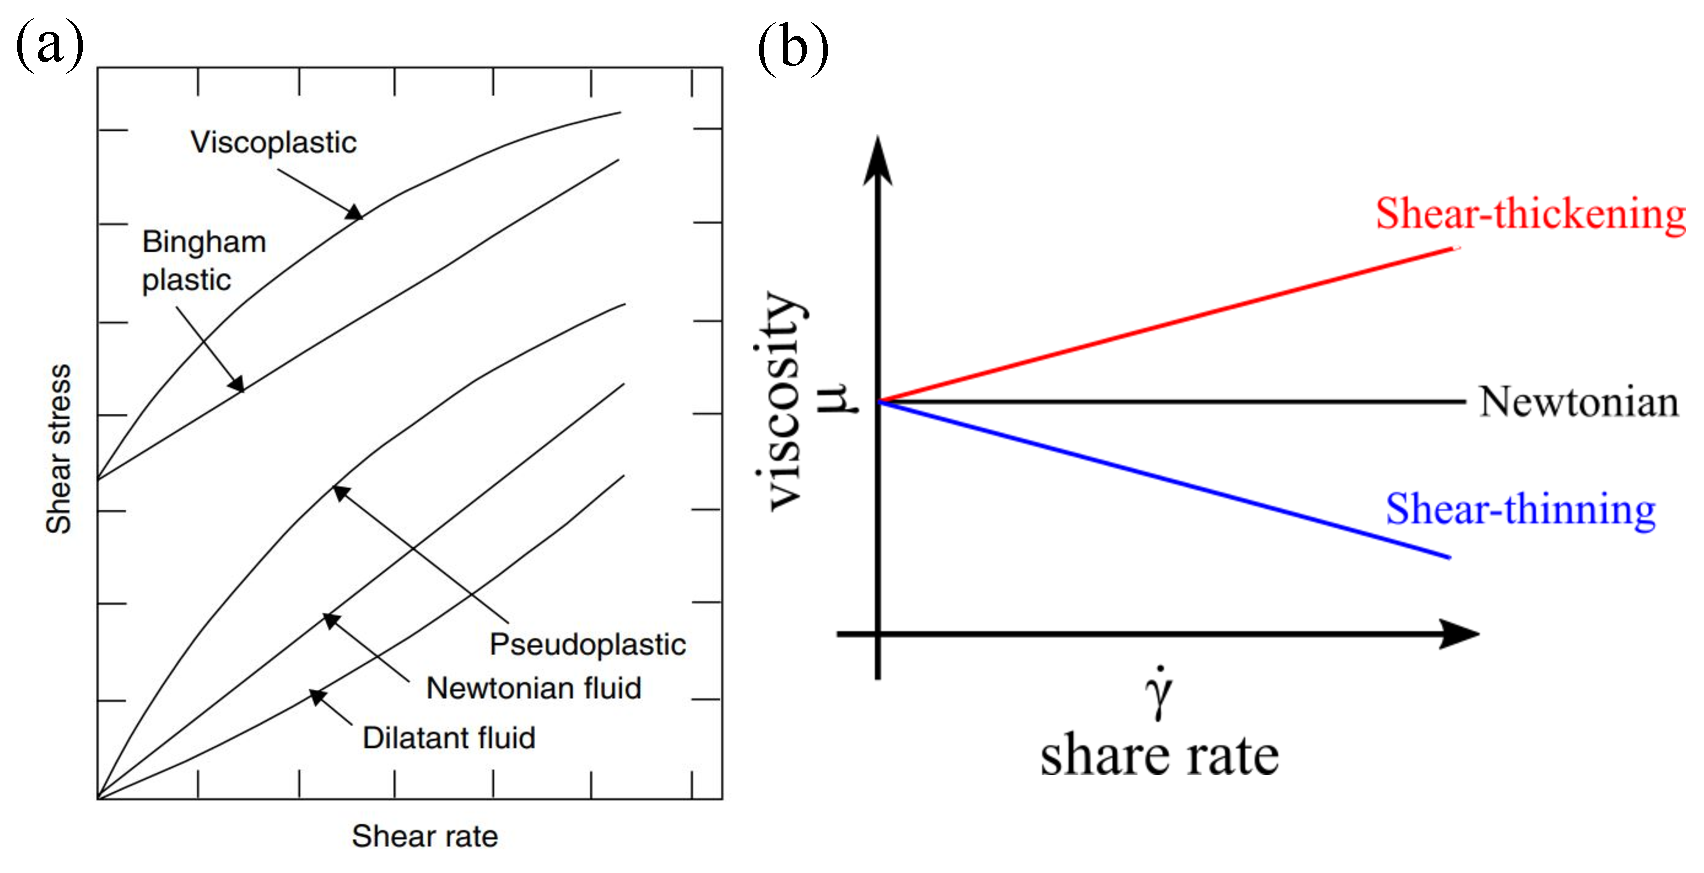
\includegraphics[width=1\textwidth]{1-Background/shea-thining.eps}
    \caption{(a) Qualitative flow curves for different types of non-Newtonian fluids\cite{ref:1}. (b)Classifications of non-Newtonian power-law fluid.}
    \label{fig:1-fluid-curve}
\end{figure}
\begin{figure}[ht]
    \begin{center}
        \includegraphics[width=12.0cm,clip]{1-Background/4-sinking.png}
        \caption{Sinking dynamics for different intruder-sizes and for different vibration intensities $\Gamma$. (a1) Depth$z$ versus time$t$ for $\dot{z}$ an intruder with radius of 4mm and (a2) for an intruder with radius of 7mm. (b1) Instantaneous velocity versus sinking depth $z$ obtained from (a1) and (b2) from (a2). The black lines correspond to the solutions fitted in the quasi-steady regime\cite{ref:6}.}
        \label{fig:4-sinking}
    \end{center}
\end{figure}
\newpage
\subsection{研究目的}

先行研究\cite{ref:8}において,超音波照射された擬塑性流体中を落下する球の高速化の要因として,音響境界層内部における粘度低下と,音響境界層の形成が関係していることが提案されている.また,高速化が弾性によって抑制されることが示唆されている.しかし,調査された流体や落下球の種類,径は限定的であり,弾性が高速化を抑制することは検証が十分ではない.落下球の密度や濃度密度を大きく変化させることで,球の周囲に生じる応力を変化させ,粘性と弾性それぞれ影響を明らかにすることができる.

本研究で用いた試験溶液では,球の落下による運動が高速の場合,粘性による影響が支配的であり,低速の場合は弾性による影響が支配的となる.落下球の終端速度を変化させることで粘性が支配的な場合と弾性が支配的な場合に分けて,超音波照射による高速化への影響を調査した.そこで,流体物性,落下物体の密度,落下球の径をより大きく変化させ実験を行った.超音波照射された擬塑性流体中を落下する球の高速化に対する粘弾性両方の影響を明らかにすることを目的とする.

\newpage
\section{落下球高速化の理論}

擬塑性流体中における球の落下メカニズムより考える.代表速度,代表長さとして,それぞれ,落下速度$U_T$,球直径$2a$を選ぶ.また,power-law (式(\ref{eq:power-low}))に従う流体の代表粘度を$k U_T/(2a)$とする.これらより,粒子レイノルズ数は次式で与えられる\cite{ref:1},\cite{ref:8-5}.
\begin{eqnarray}
    Re = \frac{\rho_1 \left(2a\right)^n U_T^{2-n}}{k} ,
\end{eqnarray}
と表される\cite{ref:1,ref:8-5}.今回の実験結果より,$\rho \approx$1000[kg/m${}^3$],$2a =$0.01[m],$U_T \approx$0.2[m/s],\\$k =$8.37[Pa$\cdot \text{s}^n]$,$n =$0.24であるので,$Re \approx$2.3と概算することができる.これより,粒子付近ではストークス流れに近いとみなす.流れの決定因子としては,慣性に比べて粘性が支配的であると考える.

本研究の系は,一様流れ中を半径$a$の球および,超音波の伝播が存在する系である.超音波の伝播に関して,音波の圧力変動の時間スケールは$O\left(10^{-5}\right)$sである.
一方で,球の落下現象は$O\left(10^{-2}\right)$m,$O\left(10^{0}\right)$sとなり,圧力変動の時間スケールは非常に短い.球の落下に関しては,落下時間スケールで粗視化した平均的な挙動に着目する.球周囲に存在する非圧縮性流体の単位体積の運動方程式について考える.球によって誘起される応力テンソルを$\bm{\sigma}$,流体の密度を$\rho$,速度ベクトルを$\bm{v}$,体積力を$\bm{X}$とすると,
\begin{eqnarray}
    \rho \frac{D\bm{v}}{Dt} = \bm{X} + \nabla \cdot \bm{\sigma} ,
    \label{eq:undou}
\end{eqnarray}
となる.また,非圧縮性流体を仮定しているため連続の式が成り立つ.
\begin{eqnarray}
    \nabla \cdot \bm{v} = 0 .
    \label{eq:renzoku}
\end{eqnarray}
粒子重心位置から見た移動座標系では,式(\ref{eq:undou})の左辺が,
\begin{eqnarray}
    \rho \frac{D\bm{v}}{Dt} = \frac{\partial \bm{v}}{\partial t} + \left(\bm{v} - \bm{U}_T \cdot \nabla \right) \bm{v} ,
    \label{eq:nabie}
\end{eqnarray}
と展開できる.流れは十分に発達し,定常状態であると仮定することで,式(\ref{eq:nabie})の右辺第1項の時間微分項は0となる.低レイノルズ数かつStokes近似を用いることにより,慣性項は粘性項より十分に小さいと仮定することができる.これにより,式(\ref{eq:nabie})の右辺第2項の慣性項は無視することができる.加えて,粒子周囲流体には密度差がないため,静水圧分を除いた圧力を使って応力${\bm \sigma}$と書くと,体積力${\bm X}$は0となる.これらより,式(\ref{eq:undou}), (\ref{eq:nabie})を用いると,
\begin{eqnarray}
    \nabla \cdot \sigma = 0 ,
    \label{eq:sigma-}
\end{eqnarray}
といった関係が導かれる.

ある球体領域において,ガウスの発散定理より,
\begin{eqnarray}
    \int_S{\bm{\sigma \cdot \bm{n}}}dS = \int_V{\nabla \cdot \bm{\sigma}}dV ,
    \label{eq:gaussian}
\end{eqnarray}
といった関係が成り立つ.ここで,$\bm{n}$は球領域表面に対する法線ベクトル,$S$は球の表面積,$V$は球の体積を表す.式(\ref{eq:sigma-})より,式(\ref{eq:gaussian})の右辺は0である.式(\ref{eq:sigma-}),(\ref{eq:gaussian})は任意の流体体積に関して成り立つため,球の表面($r = a$)と球外部の任意の領域($r > a$)において,以下の関係が成り立つ.
\begin{eqnarray}
    \int_{r=a}\bm{\sigma}\cdot\bm{e}_r dS=\int_r\bm{\sigma}\cdot\bm{e}_r dS .
    \label{eq:inte}
\end{eqnarray}
ここで,$\bm{n} = \bm{e}_r$とする.この式は,任意の領域において,面積力が釣り合うことを示す.$r = a$における時間平均応力を$\langle\sigma\rangle_a$,$r$における時間平均応力を$\langle\sigma\rangle_r$とそれぞれする.球の表面積$S=4\pi r^2$であるので,式(\ref{eq:inte})は,
\begin{eqnarray}
    4\pi a^2\langle\sigma\rangle_a = 4\pi r^2\langle\sigma\rangle_r ,
    \label{eq:sigma1}
\end{eqnarray}
となる.球表面において,球の体積力と表面力は釣り合うので,
\begin{eqnarray}
    4\pi a^2\langle\sigma\rangle_a = \frac{4}{3} \pi a^3 \Delta \rho g ,
    \label{eq:sigma2}
\end{eqnarray}
となる.ここで,球と流体の密度差$\Delta \rho$,重力加速度$g$である.式(\ref{eq:sigma1}),(\ref{eq:sigma2})より,
\begin{eqnarray}
    \langle\sigma\rangle_r = \frac{a^3\Delta\rho g}{3r^2} ,
\end{eqnarray}
となる.低レイノルズ数で粘性項が支配的であるため,
\begin{eqnarray}
    \langle\sigma\rangle_r \sim \mu \dot{\gamma} ,
    \label{eq:sigma3}
\end{eqnarray}
と概算することができる.Power-law modelが適用できる領域での議論を行っているため,式(\ref{eq:power-low}),(\ref{eq:sigma3})より,
\begin{eqnarray}
    \dot{\gamma} \sim \left(\frac{a^3\Delta\rho g}{3r^2 k}\right)^{\frac{1}{n}} ,
    \label{eq:gamma_abs}
\end{eqnarray}
と概算される.この系において,エネルギー散逸に関して考える.位置エネルギーと粘性によるエネルギー散逸が釣り合うため,単位時間あたりに系全体が失うエネルギーバランスより,以下の式が成立する.
\begin{eqnarray}
    \int_{r>a}\bar{\epsilon}dV = 4 \pi \int^\infty_a \bar{\epsilon}r^2 dr = \frac{4}{3}\pi a^3\Delta\rho g U_T ,
    \label{eq:eg}
\end{eqnarray}
ここで,$U_T$は球の終端速度,$\bar{\epsilon}$は時間平均された単位体積当たりのエネルギー散逸である.また,粘性散逸$\bar{\epsilon}$は,以下の様に概算される.
\begin{eqnarray}
    \bar{\epsilon} \sim \langle\sigma\rangle_r\dot{\gamma} \sim \mu \dot{\gamma}^2 \sim \frac{\langle\sigma\rangle_r^2}{\mu} ,
    \label{eq:eps}
\end{eqnarray}
式(\ref{eq:sigma3}),(\ref{eq:eg}),(\ref{eq:eps})より,終端速度は
\begin{eqnarray}
    U_T \sim \frac{a^3\Delta\rho g}{3}\int_a^\infty\frac{dr}{\mu r^2} ,
    \label{eq:UT0}
\end{eqnarray}
と見積もられる.式(\ref{eq:power-low}),(\ref{eq:gamma_abs}),(\ref{eq:UT0})より,終端速度は下記の様に書き直される.
\begin{eqnarray}
    U_T \sim \frac{a^3\Delta\rho g}{3}  \int^{\infty}_{a} \frac{dr}{\mu r^2} \sim \left(\frac{\Delta \rho g}{3k}\right)^{\frac{1}{n}}\frac{n}{2-n}a^{\frac{n+1}{n}} .
    \label{eq:UT}
\end{eqnarray}

\newpage
\chapter{実験方法}
\section{概要}
本実験では,0.5,1wt.\% ポリアクリルアミド(PAA)溶液(三菱ケミカル,AP805C)を擬塑性流体としてそれぞれ用いた.また,対照実験として水道水も用いた.作製したPAA溶液が適切なものであるか評価を行うため,非ニュートン流体における指標の一つとなる粘度の計測を行った.続いて,擬塑性流体に対する超音波照射による影響の密度依存性を調べるため,様々な落下球を用いて球落下実験行った.

\section{粘度計測}
粘度計測における計測機器の模式図を\ref{fig:viscosity}に示す.ステージと回転する円錐回転子の間に存在する試料によって付加されるトルクを計測することで粘度の計測を行う.粘度のせん断速度依存性を確認することで生成した溶液の性質の確認を行った.なお、計測範囲の都合上、水道水では

\begin{center}
    \begin{figure}[h]
        \includegraphics[clip,width=8.0cm]{2-Methods/Viscosity-Measurement.png}
        \caption{Viscosity measurement method.}
        \label{fig:viscosity}
    \end{figure}
\end{center}

\section{球落下実験}

使用した実験装置の概略図を\ref{device}に示す.外寸において高さ255mm,幅50mm,奥行き50mm,厚さ5mmの矩形アクリル水槽に試験溶液を満たした.その上に落下球把持用のピックアップツールをマグネットベースによって固定した.
% TODO:水槽外寸計測
\begin{center}
    \begin{figure}[H]
        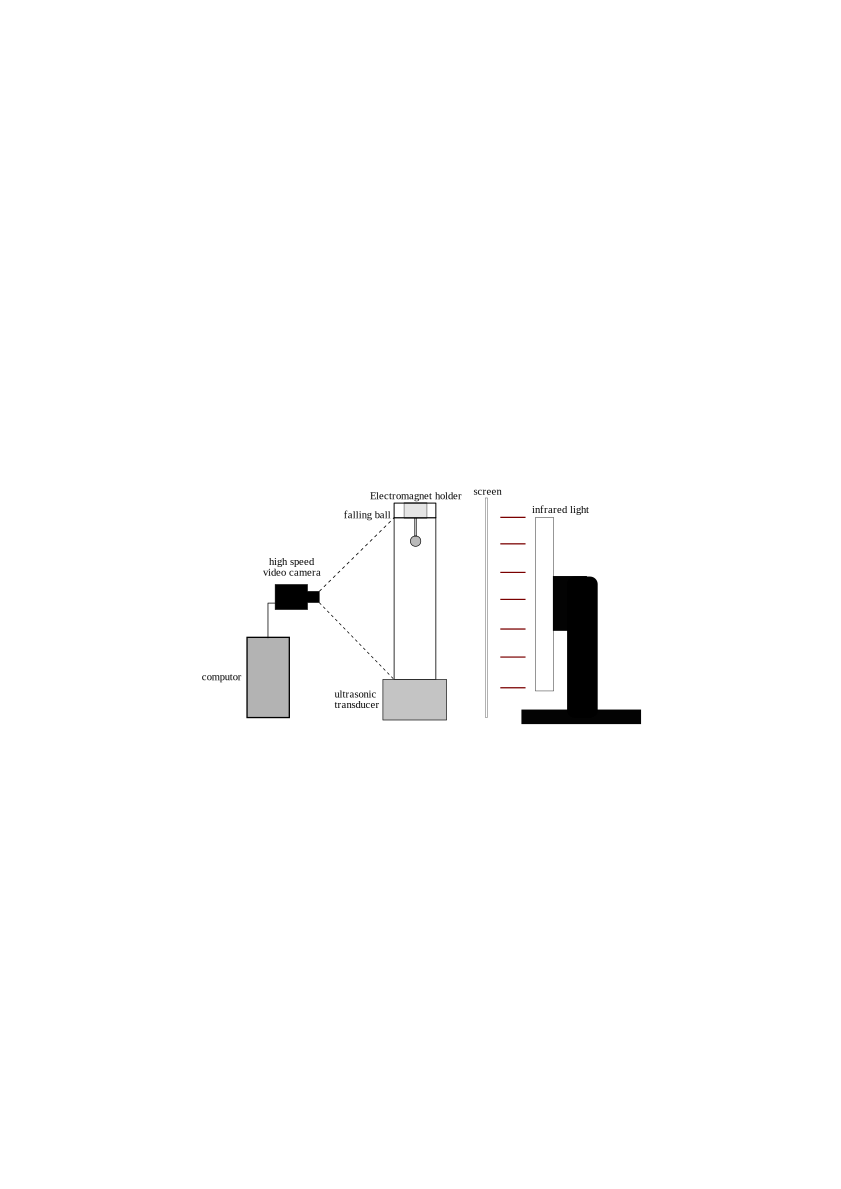
\includegraphics[clip,width=15.0cm]{2-Methods/device.png}
        \caption{Schematic view of the experimental apparatus.}
        \label{fig:device}
    \end{figure}
\end{center}

\newpage
\chapter{解析方法}
ハイスピードカメラを用いて落下球が落下する様子をbmp形式の連続画像として撮影するとFig.\ref{fig:expPhoto}(a) に示すように落下球以外にも電磁石や水槽壁面が存在する.この画像から,落下球を検出するためにHough変換を用いた.しかし,Hough変換は任意の幾何形状を表す円に対して特徴点に対して一定数以上通る円を検出する変換手法であるため,球の輪郭が必要となる.本実験では落下球の輪郭を描く方法として背景処理とSobel filterを用いた.
\section{背景処理とSobel filter}
Hough変換を行う前処理として,背景処理とSobel filterの処理を行った.撮影した連続画像に背景処理を行うとFig.\ref{fig:expPhoto}(b) に示すようになった.背景処理では,画像輝度値の平均値をとり,それぞれの画像との差分を取り,それぞれの画像における差分を明確にした.続いて,背景処理を行った画像へSobel filterの処理を行った.Sobel filterとは,輪郭抽出を行うフィルタ処理である.具体的な処理として,ある任意の画素を中心とした9つの輝度値に対し,Fig.\ref{fig:sobel}(a)(b)に示す係数をそれぞれ乗算し合計した後,絶対値をとる.Fig.\ref{fig:sobel}(a)よりy軸方向の輪郭を,Fig.\ref{fig:sobel}(b) よりx軸方向の輪郭を強調する.Fig.\ref{fig:sobel}(a)(b)それぞれによって,フィルタ処理された9つの輝度値に対する乗算の合計値を2乗し,足し合わせた後に平方することで平均をとった.Sobel filter処理後の画像をFig.\ref{fig:expPhoto}(c) に示す.

\begin{figure}[h]
    \centering
    \includegraphics[width=5.0cm,clip]{3-Analysis/exp-img.png}
    \caption{(a) Original image, (b) Image used by background processing and, (c) Image used by Sobel filter.}
    \label{fig:expPhoto}
\end{figure}

\begin{figure}[h]
    \centering
    \includegraphics[width=7.0cm,clip]{3-Analysis/sobel-filter.png}
    \caption{(a) Horizonal (b) Vertical Sobel filter.}
    \label{fig:sobel}
\end{figure}

\section{Hough変換による円の検出}
背景処理とSobel filter処理を行った画像内から鋼球の検出を行うために,Hough変換による円検出を用いた.検出手順は,以下に示す通りである.円は中心座標と半径により一意に定まる.このことより,円の中心座標 ($x_c$, $y_c$) ,半径r による1つの円D ($x_c$, $y_c$, r) に関して考える.

\begin{figure}[h]
    \centering
    \includegraphics[width=7.0cm,clip]{3-Analysis/hough.PNG}
    \caption{Outline of Hough transform.}
    \label{fig:hough}
\end{figure}

\newpage
\section{実験結果}
\subsection{粘度計測}
鋼球落下実験を行う試験溶液として,1wt.\%PAA溶液の製作を行った.この製作した溶液の粘度特性を確認し,先行研究\cite{ref:9}\cite{ref:10}における粘度特性と比較した.この比較を行うことで先行研究との粘度特性の違いを確認した.なお,この粘度計測を実施するためには,溶質が溶媒に十分に均一に溶解することならびに,混合時に混入した気泡がおおむね消失することが必要であるため,溶液製作1週間後に行った.それぞれの試料に対し,円錐回転子の回転数を変化させ,各5回計測を行いその平均を求めた.

水道水の粘度計測を行った結果をFig.\ref{fig:water-vis}に示す.なお,縦軸は粘度,横軸はせん断速度を表す.2.2においても示したが,コーンロータの回転速度を変化させることにより,せん断速度を変化させた.その結果,粘度は約1.1$\left[Pa\times s\right]$でほぼ一定となっていた.これは,水がニュートン流体であり,粘度を比例係数とした速度勾配とせん断応力の比例関係となっているためであると考えられる.

水道水の場合と同様にPAA溶液の粘度計測を行った結果をFig.\ref{fig:PAA-vis}に示す.なお,縦軸は粘度の対数,横軸はせん断速度の対数を表す.また,Iwamuro {\it et al.}\cite{ref:9}やShiratori {\it et al.}\cite{ref:10}の文献値も共に示した.ここで,粘度$\mu$はせん断速度$\dot{\gamma}$に対して,粘度定数 k[Pa$\times s^n$],指数$n$を用いthe Power-law modelに従うものとすると,
\begin{eqnarray}
    \label{eq:power-low}
    \mu=k\times\dot{\gamma}^{n-1}
\end{eqnarray}
といった式で与えられる\cite{ref:1}.式\ref{eq:power-low}を用いて近似線計算を行った結果,$k=7.39[Pa\times s^n]$,$n=0.23$であった.Iwamuro {\it et al.}\cite{ref:9}では,$k=9.4[Pa\times s^n]$,$n=0.23$と示されている.また,Shiratori {\it et al.}\cite{ref:10}を同様に解析すると,$k$=4.7[Pa$\times s^n$],$n=0.18$となっていた.今回作製したPAA溶液の粘度特性はIwamuro {\it et al.}とShiratori {\it et al.}の間に位置しており,適切に作製されたと判断できる.

\begin{figure}[ht]
    \centering
    \includegraphics[width=12cm,clip]{4-Results/water.png}
    \caption{Meansured viscosity versus shear rate for tap water.}
    \label{fig:water-vis}
\end{figure}

\begin{figure}[ht]
    \centering
    \includegraphics[width=12cm,clip]{4-Results/PAA-viscosity.png}
    \caption{Flow curve for 1wt.\%PAA solution.}
    \label{fig:PAA-vis}
\end{figure}

\newpage

\subsection{圧力場 計測結果}

0.5wt.\%PAA溶液における超音波圧力場の計測を行った結果をFig.\ref{fig:pressure}(a)に示す.また,1wt.\%PAA溶液における超音波圧力場の計測を行った結果をFig.\ref{fig:pressure}(b)に示す.縦軸は水槽底面からの高さ,横軸は圧力である.この結果を元にTable.\ref{table:press}に圧力$P$のy方向平均値を示す.Iwamuro {\it et al.}\cite{ref:8}と比較して形成された圧力場が強いことが分かった.これは容器材質がIwamuro {\it et al.}\cite{ref:8}においてはガラス製であり,振動子板がSUS製であるが,今回どちらもアクリル製となっている.このことにより,超音波振動の伝達性能が向上したためだと考えられる.

\begin{table}[h]
    \centering
    \caption{Averaged value of pressure data.}
    \label{table:press}
    \begin{tabular}{c|c|c|c}\hline
                       & Present 0.5wt.\% PAA & Present 1wt.\% PAA & Iwamuro {\it et al.}\cite{ref:8} \\ \hline
        $\bar{P}$[kPa] & 97.3                 & 107.6              & 72                               \\ \hline
    \end{tabular}
\end{table}

\begin{figure}[ht]
    \centering
    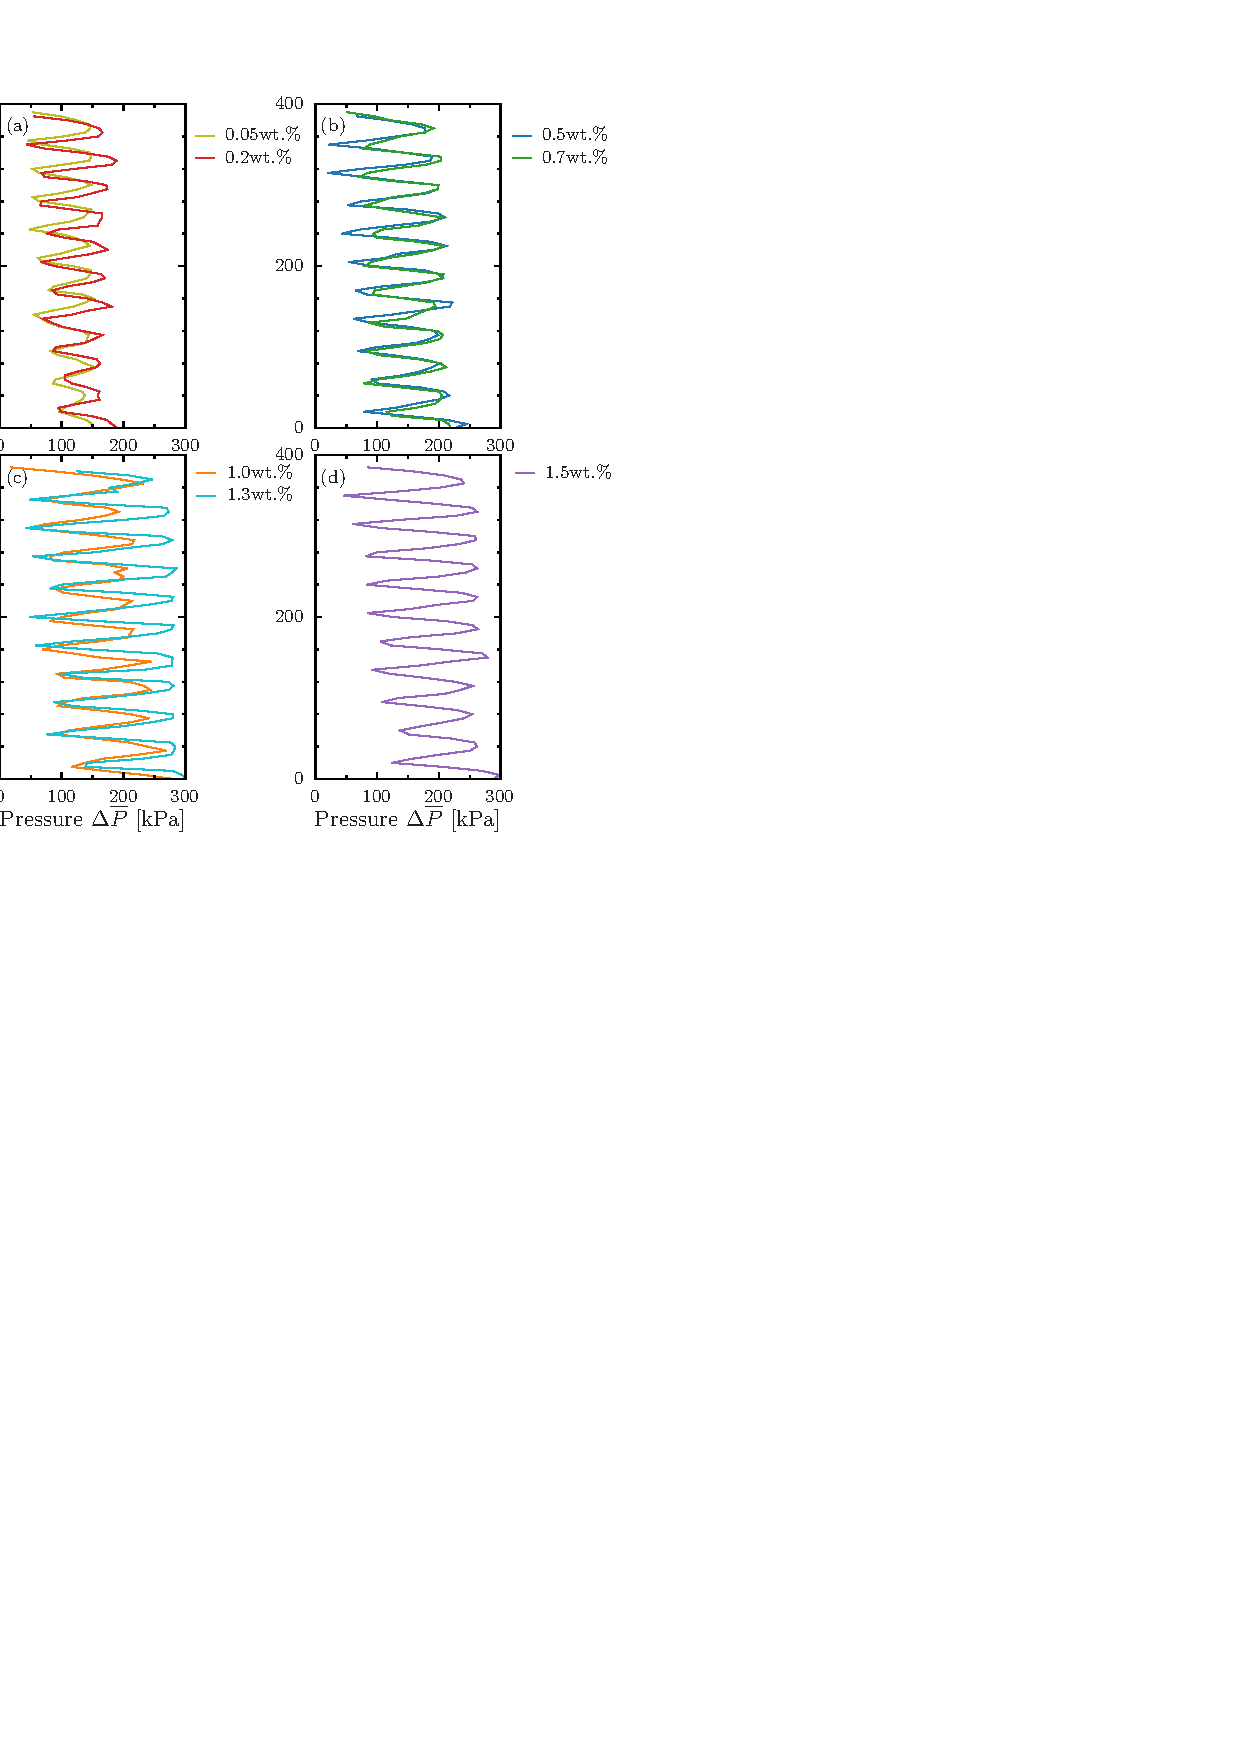
\includegraphics[width=11cm,clip]{4-Results/press.png}
    \caption{Pressure field in PAA solution measurement results.}
    \label{fig:pressure}
\end{figure}

\newpage

\subsection{落下球実験結果}

水道水中における球の落下速度を解析した結果をFig.\ref{fig:water}に示す.縦軸は落下速度,横軸は落下開始時からの経過時間である.この結果からもわかる通り,水道水中において超音波照射の有無による球の落下速度の変化は発生しなかった.

1wt.\%PAA溶液中における球の落下速度を解析した結果をFig.\ref{fig:1PAA-falling}に示す.縦軸は落下速度,横軸は落下開始時からの経過時間である.先行研究であるIwamuro {\it et al.}\cite{ref:9}と比較して,超音波照射有無に関せず速度が増加している.これは粘度が低いためであると考えられる.また,超音波照射時における加速がIwamuro {\it et al.}\cite{ref:9}と比較して大きくなっている.このことは先述の4.2にて示した通り,今回形成された圧力場がより強いためであると考えられる.同様に0.5wt.\%PAA溶液中における球の落下速度を解析した結果をFig.\ref{fig:0.5PAA-falling}に示す.縦軸は落下速度,横軸は落下開始時からの経過時間である.
\newpage
\begin{figure}[ht]
    \centering
    \includegraphics[width=12cm,clip]{./4-Results/f-water.png}
    \caption{Velocity of a falling sphere with a diameter of 2.4mm in water with or without ultrasound irradiation.}
    \label{fig:water}
    \centering
    \includegraphics[width=12cm,clip]{./4-Results/s0.5.png}
    \caption{Velocity of a falling sphere in 0.5wt.\%PAA solution for various frequency of
        ultrasound irradiation.}
    \label{fig:0.5PAA-falling}
    \centering
    \includegraphics[width=12cm,clip]{./4-Results/s1.png}
    \caption{Velocity of a falling sphere in 1wt.\%PAA solution for various frequency of
        ultrasound irradiation.}
    \label{fig:1PAA-falling}
\end{figure}

\clearpage
\section{実験装置改良により生じた変化}

\subsection{落下実験結果}

容器Aにおいて,真空ポンプを用いて球を落下させた.解析した結果をFig\ref{fig:falling-A}に示す.縦軸は落下速度,横軸は落下開始時からの経過時間である.先行研究であるIwamuro \textit{et al}.\cite{ref:8}や電磁石を用いて球を把持した場合と比較し,超音波照射による高速化が顕著に現れていないことが分かる.また,落下開始時に電磁石を用いた場合はオーバーシュートが見られるが,真空ポンプを用いた場合はオーバーシュートが見られなかった.このことに関して,後述の第\ref{sec:dis-de}節にて議論を行う.また,補足資料\ref{sec:reexp}に真空ポンプを用いた把持方法における再現性の確認結果を示す.

\begin{figure}[ht]
    \centering
    \includegraphics[width=12cm,clip]{./4-Results/s1-A.png}
    \caption{Falling speed of a sphere in 1wt.\%PAA solution with and without ultrasound irradiation in tank A.}
    \label{fig:falling-A}
\end{figure}

\subsection{実験装置改良に伴う終端速度の変化}

Iwamuro\cite{ref:8}と比較して,真空ポンプを用いて落下球を把持した場合,超音波照射のない状態において落下速度が大きかった.このことに関して,擬塑性流体中における球の落下メカニズムより考える.代表速度,代表長さとして,それぞれ,落下速度$U_T$,球直径$2a$を選ぶ.また,power-law (式(\ref{eq:power-low}))に従う流体の代表粘度を$k U_T/(2a)$とする.これらより,粒子レイノルズ数は次式で与えられる\cite{ref:1},\cite{ref:8-5}.
\begin{eqnarray}
    Re = \frac{\rho_1 \left(2a\right)^n U_T^{2-n}}{k} ,
\end{eqnarray}
と表される\cite{ref:1,ref:8-5}.今回の実験結果より,$\rho \approx$1000[kg/m${}^3$],$2a =$0.01[m],$U_T \approx$0.2[m/s],\\$k =$8.37[Pa$\cdot \text{s}^n]$,$n =$0.24であるので,$Re \approx$2.3と概算することができる.これより,粒子付近ではストークス流れに近いとみなす.流れの決定因子としては,慣性に比べて粘性が支配的であると考える.

本研究の系は,一様流れ中を半径$a$の球および,超音波の伝播が存在する系である.超音波の伝播に関して,音波の圧力変動の時間スケールは$O\left(10^{-5}\right)$sである.
一方で,球の落下現象は$O\left(10^{-2}\right)$m,$O\left(10^{0}\right)$sとなり,圧力変動の時間スケールは非常に短い.球の落下に関しては,落下時間スケールで粗視化した平均的な挙動に着目する.球周囲に存在する非圧縮性流体の単位体積の運動方程式について考える.球によって誘起される応力テンソルを$\bm{\sigma}$,流体の密度を$\rho$,速度ベクトルを$\bm{v}$,体積力を$\bm{X}$とすると,
\begin{eqnarray}
    \rho \frac{D\bm{v}}{Dt} = \bm{X} + \nabla \cdot \bm{\sigma} ,
    \label{eq:undou}
\end{eqnarray}
となる.また,非圧縮性流体を仮定しているため連続の式が成り立つ.
\begin{eqnarray}
    \nabla \cdot \bm{v} = 0 .
    \label{eq:renzoku}
\end{eqnarray}
粒子重心位置から見た移動座標系では,式(\ref{eq:undou})の左辺が,
\begin{eqnarray}
    \rho \frac{D\bm{v}}{Dt} = \frac{\partial \bm{v}}{\partial t} + \left(\bm{v} - \bm{U}_T \cdot \nabla \right) \bm{v} ,
    \label{eq:nabie}
\end{eqnarray}
と展開できる.流れは十分に発達し,定常状態であると仮定することで,式(\ref{eq:nabie})の右辺第1項の時間微分項は0となる.低レイノルズ数かつStokes近似を用いることにより,慣性項は粘性項より十分に小さいと仮定することができる.これにより,式(\ref{eq:nabie})の右辺第2項の慣性項は無視することができる.加えて,粒子周囲流体には密度差がないため,静水圧分を除いた圧力を使って応力${\bm \sigma}$と書くと,体積力${\bm X}$は0となる.これらより,式(\ref{eq:undou}), (\ref{eq:nabie})を用いると,
\begin{eqnarray}
    \nabla \cdot \sigma = 0 ,
    \label{eq:sigma-}
\end{eqnarray}
といった関係が導かれる.

ある球体領域において,ガウスの発散定理より,
\begin{eqnarray}
    \int_S{\bm{\sigma \cdot \bm{n}}}dS = \int_V{\nabla \cdot \bm{\sigma}}dV ,
    \label{eq:gaussian}
\end{eqnarray}
といった関係が成り立つ.ここで,$\bm{n}$は球領域表面に対する法線ベクトル,$S$は球の表面積,$V$は球の体積を表す.式(\ref{eq:sigma-})より,式(\ref{eq:gaussian})の右辺は0である.式(\ref{eq:sigma-}),(\ref{eq:gaussian})は任意の流体体積に関して成り立つため,球の表面($r = a$)と球外部の任意の領域($r > a$)において,以下の関係が成り立つ.
\begin{eqnarray}
    \int_{r=a}\bm{\sigma}\cdot\bm{e}_r dS=\int_r\bm{\sigma}\cdot\bm{e}_r dS .
    \label{eq:inte}
\end{eqnarray}
ここで,$\bm{n} = \bm{e}_r$とする.この式は,任意の領域において,面積力が釣り合うことを示す.$r = a$における時間平均応力を$\langle\sigma\rangle_a$,$r$における時間平均応力を$\langle\sigma\rangle_r$とそれぞれする.球の表面積$S=4\pi r^2$であるので,式(\ref{eq:inte})は,
\begin{eqnarray}
    4\pi a^2\langle\sigma\rangle_a = 4\pi r^2\langle\sigma\rangle_r ,
    \label{eq:sigma1}
\end{eqnarray}
となる.球表面において,球の体積力と表面力は釣り合うので,
\begin{eqnarray}
    4\pi a^2\langle\sigma\rangle_a = \frac{4}{3} \pi a^3 \Delta \rho g ,
    \label{eq:sigma2}
\end{eqnarray}
となる.ここで,球と流体の密度差$\Delta \rho$,重力加速度$g$である.式(\ref{eq:sigma1}),(\ref{eq:sigma2})より,
\begin{eqnarray}
    \langle\sigma\rangle_r = \frac{a^3\Delta\rho g}{3r^2} ,
\end{eqnarray}
となる.低レイノルズ数で粘性項が支配的であるため,
\begin{eqnarray}
    \langle\sigma\rangle_r \sim \mu \dot{\gamma} ,
    \label{eq:sigma3}
\end{eqnarray}
と概算することができる.Power-law modelが適用できる領域での議論を行っているため,式(\ref{eq:power-low}),(\ref{eq:sigma3})より,
\begin{eqnarray}
    \dot{\gamma} \sim \left(\frac{a^3\Delta\rho g}{3r^2 k}\right)^{\frac{1}{n}} ,
    \label{eq:gamma_abs}
\end{eqnarray}
と概算される.この系において,エネルギー散逸に関して考える.位置エネルギーと粘性によるエネルギー散逸が釣り合うため,単位時間あたりに系全体が失うエネルギーバランスより,以下の式が成立する.
\begin{eqnarray}
    \int_{r>a}\bar{\epsilon}dV = 4 \pi \int^\infty_a \bar{\epsilon}r^2 dr = \frac{4}{3}\pi a^3\Delta\rho g U_T ,
    \label{eq:eg}
\end{eqnarray}
ここで,$U_T$は球の終端速度,$\bar{\epsilon}$は時間平均された単位体積当たりのエネルギー散逸である.また,粘性散逸$\bar{\epsilon}$は,以下の様に概算される.
\begin{eqnarray}
    \bar{\epsilon} \sim \langle\sigma\rangle_r\dot{\gamma} \sim \mu \dot{\gamma}^2 \sim \frac{\langle\sigma\rangle_r^2}{\mu} ,
    \label{eq:eps}
\end{eqnarray}
式(\ref{eq:sigma3}),(\ref{eq:eg}),(\ref{eq:eps})より,終端速度は
\begin{eqnarray}
    U_T \sim \frac{a^3\Delta\rho g}{3}\int_a^\infty\frac{dr}{\mu r^2} ,
    \label{eq:UT0}
\end{eqnarray}
と見積もられる.式(\ref{eq:power-low}),(\ref{eq:gamma_abs}),(\ref{eq:UT0})より,終端速度は下記の様に書き直される.
\begin{eqnarray}
    U_T \sim \frac{a^3\Delta\rho g}{3}  \int^{\infty}_{a} \frac{dr}{\mu r^2} \sim \left(\frac{\Delta \rho g}{3k}\right)^{\frac{1}{n}}\frac{n}{2-n}a^{\frac{n+1}{n}} .
    \label{eq:UT}
\end{eqnarray}

上記の式(\ref{eq:UT})より,Power-Law modelにおける,$k$,$n$のパラメータより終端速度を見積もることができる.ここで,溶液の作製誤差に関して考えるため,0.95wt.\%,1.05wt.\%のPAA溶液を同様の手順で作製した.粘度計測を行った結果をFig.\ref{fig:95-105}に示す.濃度が薄いと粘度は低く,濃度が高いと粘度は高くなった.

Table \ref{table:power-law}の結果より,式(\ref{eq:UT})を用いて直径10mmの球におけるIwamuro\cite{ref:8}の終端速度$U_I$を基準とした終端速度の比$U_T/U_{I}$を求めた.その結果を,Table \ref{table:UT}に示す.これより,今回の粘度特性において,Iwamuro\cite{ref:8}と比較して終端速度が1.09倍速くなることが分かった.Fig.\ref{fig:falling-A}において,Iwamuro\cite{ref:8}と比較して1.125倍,終端速度が速かった.一方で,0.95,1.05wt.\%それぞれのPAA溶液の粘度特性における終端速度比と比較しても実験結果と一番近いのは,1wt.\%の場合である.よって,溶液の濃度精度は1wt.\%±0.05wt.\%以内であり,溶液の作製誤差によって落下速度に差が生じたと考えられる.

\begin{figure}[ht]
    \includegraphics[width=15cm,clip]{5-Discussion/95-105.png}
    \caption{Flow curve for 0.95~1.05wt.\%PAA solution.}
    \label{fig:95-105}
\end{figure}

\begin{table}[h]
    \centering
    \caption{Each parameter($k$,$n$) and terminal speed ratio in the power-law model for each experimental result.}
    \label{table:UT}
    \begin{tabular}{c|c|c|c} \hline
        & $k$ & $n$ & $U_T/U_{I}$ \\ \hline \hline
        Present Value(1.05wt.\%) & 9.56 & 0.23 & 0.93\\
        Present Value(1wt.\%) & 8.37 & 0.24 & 1.09\\
        Present Value(0.95wt.\%) & 5.22 & 0.25 & 3.91\\
        Iwamuro\cite{ref:8} & 9.4 & 0.23 & 1\\
        Shiratori \textit{et al}.(2016)\cite{ref:10} & 5.9 & 0.25 & 2.99\\ \hline
    \end{tabular}
\end{table}

\newpage

\subsection{落下開始時のオーバーシュートへの影響}
\label{sec:dis-de}

今回,球を把持する手法を,電磁石を用いて把持する方法から真空ポンプを用いて把持する方法に変化させた.この時,落下開始時0-0.3sにおける落下速度のオーバーシュートが,先行研究\cite{ref:8,ref:9}より小さくなった.落下開始時のオーバーシュートは弾性による影響によって生じる\cite{ref:12}.以下で,オーバーシュートが見られなくなった原因を,物質の流動性を表す$De$数より考える.$De$数が大きくなると,弾性的傾向が強くなり,$De$数が小さくなると,粘性的流動を表す.

$De$数は下記の様に緩和時間$\lambda$[s],代表時間$T$[s]の比で表される.
\begin{equation}
    De = \frac{\lambda}{T} .
    \label{eq:De}
\end{equation}
代表時間$T$[s]に関して,超音波照射を行っていない場合の球の落下条件においても考えるため,
\begin{equation}
    T = \frac{a}{U} ,
    \label{eq:T}
\end{equation}
となる.ここで,球の落下速度$U$[m/s],球の半径$a$[m]である.また,緩和時間$\lambda$[s]は,
\begin{equation}
    \lambda \approx \frac{\mu}{G'} .
    \label{eq:lamda}
\end{equation}
ここで粘度$\mu$[Pa$\times$s],貯蔵弾性率$G'$[Pa]である.緩和時間は変形の経過時間において,粘弾性流体が流体的挙動を示すか,固体的挙動を示すかの指標である\cite{ref:sakanishi}.粘度$\mu$[Pa$\times$s]に関して,せん断速度$\dot{\gamma}$[1/s]および粘度定数$k$[Pa$\times$s${}^n$],指数$n$を用いてPower-law modelに従うとすると,
\begin{equation}
    \mu = k \times \dot{\gamma}^{n-1} ,
    \label{eq:power-law}
\end{equation}
となる.落下球によるせん断領域において,せん断速度の代表値$\dot{\gamma}$[1/s]は,次のように概算される.
\begin{equation}
    \dot{\gamma} \sim \frac{U}{a} .
    \label{eq:gamma}
\end{equation}
よって,式(\ref{eq:power-law}),(\ref{eq:gamma})よりせん断領域における粘度$\mu_U$は,次式で概算される.
\begin{equation}
    \mu_U \sim k \times \left(\frac{U}{a}\right)^{n-1} .
    \label{eq:power-law2}
\end{equation}
これら式(\ref{eq:De}),(\ref{eq:T}),(\ref{eq:lamda}),(\ref{eq:power-law2})より,$De$数は,
\begin{equation}
    De \sim \frac{k}{G'} {\left(\frac{U}{a}\right)}^n ,
    \label{eq:De2}
\end{equation}
となり,粘度定数$k$[Pa$\times$s${}^n$],貯蔵弾性率$G'$[Pa],落下速度$U$[m/s],球の半径$a$[m]によって表される.

貯蔵弾性率$G'$[Pa]に関して,先行研究において計測されたFig.\ref{fig:iwamuro-G}(b)の結果より考える.この図において,貯蔵弾性率$G'$[Pa]は応力$\tau$[Pa]との関係性が示されている.ここで応力$\tau$[Pa]は,
\begin{equation}
    \tau = \mu \times \dot{\gamma} ,
    \label{eq:tau}
\end{equation}
となる.ここに,式(\ref{eq:power-law}),(\ref{eq:gamma})を代入すると,
\begin{equation}
    \tau \sim k \times \left(\frac{U}{a}\right)^n , 
    \label{eq:tau-cal}
\end{equation}
と概算することができる.

Fig.\ref{fig:falling-A}, \ref{fig:iwamuro-fall}それぞれの結果より,ピーク速度$U_{peak}$[mm/s]と終端速度$U_{ave}$[mm/s]を算出した.続いて,式(\ref{eq:tau-cal})を用いて,それぞれの速度における応力$\tau_{peak}$[Pa],$\tau_{ave}$[Pa]の算出を行った.これら算出結果と先行研究の計測結果Fig.\ref{fig:iwamuro-G}より,貯蔵弾性率$G'$も求めた.これらの結果を,Table \ref{table:iwamuro}に示す.

また,式(\ref{eq:power-law2})を用いて,ピーク速度/終端速度それぞれの粘度$\mu_{peak}$[Pa$\cdot$s],$\mu_{ave}$[Pa$\cdot$s]を概算した.これらの粘度を式(\ref{eq:lamda})に代入し,それぞれの緩和時間$\lambda_{peak}$[s],$\lambda_{ave}$[s]の算出を行った.そして,それらの緩和時間より,式(\ref{eq:De})を用いて,それぞれの$De$数,$De_{peak}$,$De_{ave}$を求めた.これらの結果を,Table \ref{table:iwamuro2}に示す.

Table \ref{table:iwamuro2}より,ピーク速度より求めた$De_{peak}$と,終端速度より求めた$De_{ave}$において,大きな差異が見られないことが分かった.以降,$De_{peak}$に関してのみ議論を行う.$De_{peak}$に関して,落下速度のオーバーシュート$U_{peak}/U_{ave}$との関係をFig.\ref{fig:De-overshoot}に示す.横軸は$De$数,縦軸は落下速度のオーバーシュート$U_{peak}/U_{ave}$である.この図より,$De$数とオーバーシュートには正の相関があり,$De$数が増加するとオーバーシュートも大きくなることが分かった.

\begin{table}[hbtp]
    \caption{Peak speed $U_{peak}$/ terminal speed $U_{ave}$, stress $\tau$, storage modulus $G'$ Calculation result.}
    \label{table:iwamuro}
    \centering
    \begin{tabular}{ccccccc}
      \hline
      \multirow{2}{*}{実験者} & 球直径[mm] & ピーク速度[mm/s] & 終端速度[mm/s] &\multicolumn{2}{c}{応力[Pa]} & 貯蔵弾性率[Pa] \\
       & $D=2a$ & $U_{peak}$ & $U_{ave}$ &  $\tau_{peak}$ & $\tau_{ave}$ & $G'$\\
      \hline \hline
      \multirow{8}{*}{Iwamuro} & 3  & 10.08 & 9.05 & 14.6 & 14.2 & 8\\
      & 4  & 23.2 & 19.4 & 16.5 & 15.9 & 7\\
      & 5  & 34.8 & 32.6 & 17.2 & 17.0 & 6.7 \\
      & 6  & 46.3 & 54.8 & 17.6 & 18.3 & 6.5\\
      & 7  & 79.8 & 82 & 19.3 & 19.4 & 5.5\\
      & 8  & 130 & 113 & 20.9 & 20.3 & 5 \\
      & 9  & 193 & 133 & 22.3 & 20.5 & 4\\
      & 10 & 256 & 168 & 23.2 & 21.2 & 3.5\\
      \hline \hline
      Niwa & 10 & 148 & 144 & 18.9 & 18.7 & 6 \\
      \hline
    \end{tabular}
\end{table}
\begin{table}[hbtp]
    \caption{Viscosity $\mu$, Relaxation time $\lambda$, number of $De$ Calculation result.}
    \label{table:iwamuro2}
    \centering
    \begin{tabular}{ccccccccc}
      \hline
      \multirow{2}{*}{実験者} & 球直径 &\multicolumn{2}{c}{粘度[Pa$\cdot$s]} &\multicolumn{2}{c}{緩和時間[s]}  &\multicolumn{2}{c}{$De$数[-]} \\
       & $D=2a$[mm] & $\mu_{peak}$ & $\mu_{ave}$  &  $\lambda_{peak}$ & $\lambda_{ave}$ & $De_{peak}$ & $De_{ave}$ \\
      \hline \hline
      \multirow{8}{*}{Iwamuro} & 3  & 2.17 & 2.36 & 0.27 & 0.29 & 1.82 & 1.78\\
      & 4  & 1.42 & 1.63 & 0.20 & 0.23 & 2.36 & 2.26\\
      & 5  & 1.24 & 1.30 & 0.18 & 0.19 & 2.57 & 2.53 \\
      & 6  & 1.14 & 1.00 & 0.18 & 0.15 & 2.71 & 2.82\\
      & 7  & 0.85 & 0.83 & 0.15 & 0.15 & 3.51 & 3.53\\
      & 8  & 0.64 & 0.72 & 0.13 & 0.14 & 4.19 & 4.05 \\
      & 9  & 0.52 & 0.69 & 0.13 & 0.17 & 5.58 & 5.12\\
      & 10 & 0.45 & 0.63 & 0.13 & 0.18 & 6.64 & 6.03\\
      \hline \hline
      Niwa & 10 & 0.64 & 0.65 & 0.11 & 0.11 & 3.15 & 3.12 \\
      \hline
    \end{tabular}
\end{table}

\begin{figure}[ht]
    \begin{center}
        \includegraphics[width=13cm,clip]{5-Discussion/iwamuro-fall.png}
    \caption{Speed of a falling sphere in diameter of (a) 3 mm, (b) 4 mm, (c) 5 mm, (d) 6 mm, (e) 7 mm, (f) 8 mm, (g) 9 mm, (h) 10 mm in 1.0 wt.\% PAA solution with ultrasound fixed frequency at 27.4 kHz and $\Delta \bar{P} \approx$ 180 kPa\cite{ref:8}.}
    \label{fig:iwamuro-fall}
    \end{center}
\end{figure}

\begin{figure}[ht]
    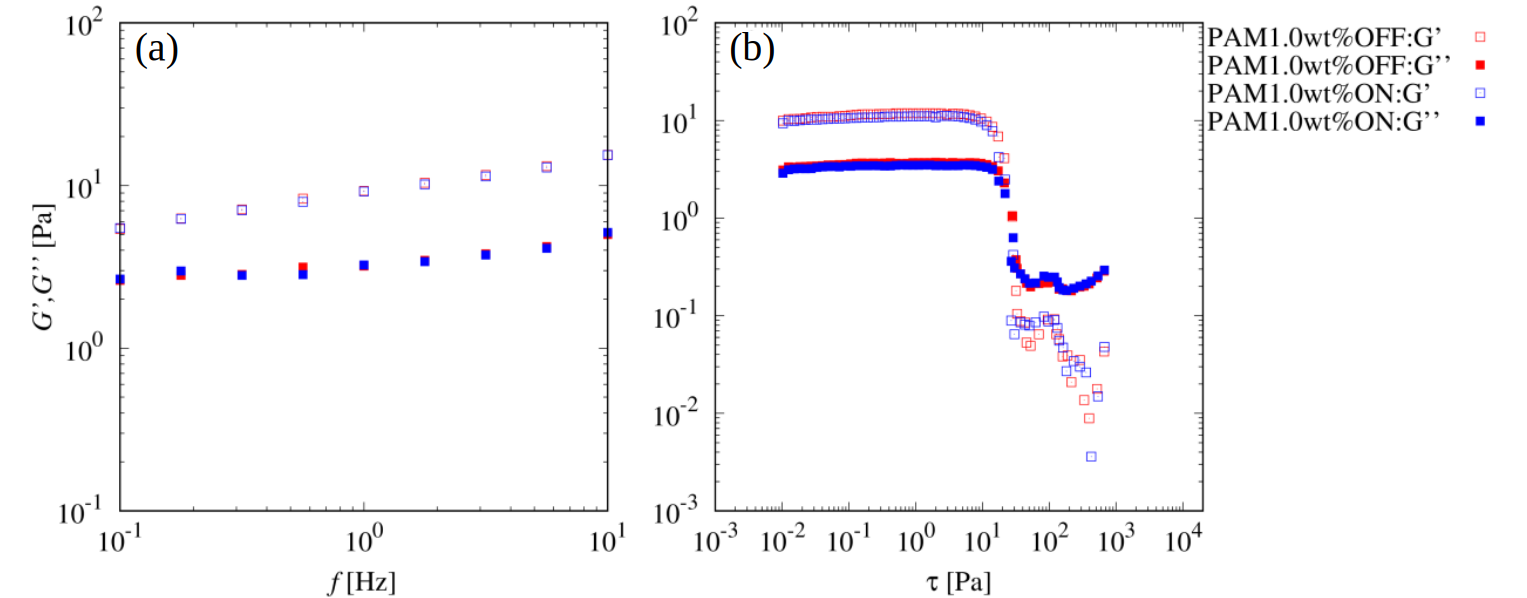
\includegraphics[width=15cm,clip]{5-Discussion/iwamuro-G.PNG}
    \caption{Frequency and stress dependence of storage and loss moduli for 1.0 wt.\% PAA.\cite{ref:8}}
    \label{fig:iwamuro-G}
\end{figure}

\begin{figure}[ht]
    \begin{center}
        \includegraphics[width=15cm,clip]{5-Discussion/De-overshoot.png}
        \caption{Relationship between overshoot $U_{peak}/U_{ave}$ and Deborah number $De$ for falling spheres.}
        \label{fig:De-overshoot}
    \end{center}
\end{figure}

\clearpage

\subsection{実験装置改良に伴う初速へ影響}

前節にて,実験装置の改良によってピーク速度が減少し,$De$が小さくなったことによってオーバーシュートが小さくなったことを示した.本節において,電磁石を用いて把持した場合,ピーク速度が大きくなった理由に関して考察を行う.電磁石を用いて球を把持した場合,電磁石へ落下方向に力を与えて落下を開始させている.この時,微小ではあるが落下開始時に初速が存在する.一方で真空ポンプを用いて球を把持した場合,吸着パッドを大気圧にすると球は落下する.この場合,球に力が加わらないため,初速は存在しない.このように初速の有無がオーバーシュートの変化に大きく関与していると考えられる.

初速の有無が与える影響に関して調査するため,真空ポンプを用いて球中心が液面より高さ$H=$5mmとなる地点で把持し,そこから球を落下させた.その結果をFig.\ref{fig:h-5}に示す.縦軸は落下速度,横軸は初速ありの場合は液面に球中心が入ったときを0s,初速なしの場合は落下開始時刻を0sとした時刻である.この条件において,初速は313[mm/s]となる.ピーク速度は440[mm/s]となり,初速を超えて加速した.これは初速と重力による加速が,粘性抵抗や浮力よりも大きく,弾性は遅れて発生するため,初速を超えて加速したと考えられる.

Iwamuro\cite{ref:9}の$a =$5[mm]における初速を推定する.この結果において,0.1sの時185[mm/s]であった.球の初速を$U_0$とすると,$U_0$の取りうる値の範囲は,0$\leqq U_0 \leqq$185[mm/s]となる.一方で,ピーク速度は256[mm/s]となり,オーバーシュートが見られた.これは,先述の初速を与えた結果と同様に弾性による影響が生じる前に初速や重力によって加速したためだと考えられる.

また,真空ポンプを用いた落下実験(niwa exp.)の$De$数は,先行研究の結果において球半径$3<a<3.5$[mm]の間における$De$数に相当した.電磁石を用いて把持した実験において,この球径においてオーバーシュートはあまり見られなかった.真空ポンプを用いた落下実験の場合,$De$数が小さくなった原因であるが,初速が存在しないため急激な速度変化とならず,ピーク速度$U_{peak}$が小さくなったためと考えられる.

よって,電磁石を用いて球を把持した場合は初速による影響がオーバーシュートとして現れるが,真空ポンプを用いて球を把持した場合は初速が非常に小さいためその影響を受けないということが分かった.

\begin{figure}[ht]
    \begin{center}
        \includegraphics[width=15cm,clip]{5-Discussion/h-5.png}
        \caption{Falling speed of a sphere in 1wt.\% PAA solution falling with initial speed.}
        \label{fig:h-5}
    \end{center}
\end{figure}
\clearpage
\section{落下球密度の影響}

\section{溶液濃度の影響}

\section{弾性による影響}

\section{落下間隔変化における高速化への寄与}
\subsection{落下実験結果}

容器Bにおいて落下間隔を5分,10分,20分と変化し,球を落下させた解析した結果をFig.\ref{fig:falling-5},\ref{fig:falling-10},\ref{fig:falling-20},に示す.縦軸は落下速度,横軸は落下開始時からの経過時間である.なお,落下間隔10分の結果に関して,比較のため先行研究であるIwamuro\cite{ref:9}における実験結果もあわせて示す.それぞれの場合において,超音波照射による落下球の高速化は見られた.

しかし,Iwamuro\cite{ref:9}と比較し,落下開始時の加速におけるオーバーシュートが今回は見られなかった.また,Iwamuro\cite{ref:9}においては落下速度は落下開始から0.8s以降,定常状態となっている.本実験において同条件である落下間隔10分において,超音波照射なしの場合,落下開始から0.2-0.7s間のみ,一定速度で落下し以降は加速した.オーバーシュートの有無は先述の装置改良における実験結果においても見られたため,実験手法の変化によるためだと考えられる.終端速度への到達の有無だが,擬塑性流体の粘弾性回復がIwamuro\cite{ref:9}と比較して十分に行われていないと考えられる.これは,落下間隔20分の条件において,Iwamuro\cite{ref:9}と同様の終端速度に達しているため,落下間隔10分では回復しきれなかった粘弾性が回復しきったためだと考えられる.粘弾性の回復時間が異なることに関しては,落下間隔をより細かく変化させ調査する必要があると考えられる.

\begin{figure}[ht]
    \centering
    \includegraphics[width=14cm,clip]{./4-Results/s1-5.png}
    \caption{Falling speed of a sphere in 1wt.\%PAA solution with and without ultrasound irradiationin tank B. (Interval 5 min.)}
    \label{fig:falling-5}
\end{figure}
\begin{figure}[ht]
    \centering
    \includegraphics[width=14cm,clip]{./4-Results/s1-10.png}
    \caption{Falling speed of a sphere in 1wt.\%PAA solution with and without ultrasound irradiationin tank B. (Interval 10 min.)}
    \label{fig:falling-10}
\end{figure}
\begin{figure}[ht]
    \centering
    \includegraphics[width=14cm,clip]{./4-Results/s1-20.png}
    \caption{Falling speed of a sphere in 1wt.\%PAA solution with and without ultrasound irradiationin tank B. (Interval 20 min.)}
    \label{fig:falling-20}
\end{figure}

\clearpage

\subsection{超音波照射による高速化}

球の落下間隔を5分,10分,20分と変化させた.その結果をFig.\ref{fig:interval-change}に示す.なお,縦軸は落下速度[mm/s],横軸は落下開始時からの経過時間[s]である.全ての条件において超音波照射に伴う高速化は見られた.また落下速度は,落下間隔10分,5分,20分の順で速かった.この結果を元に,超音波照射時の球の落下速度$U_{on}$と超音波照射なしの球の落下速度$U_{off}$として,速度比$U_{on}/U_{off}$を求めた.その結果をFig.\ref{fig:speed-diff}に示す.ここで縦軸は速度比[-],横軸は落下間隔時間[min]である.この結果より,落下速度と同様に,落下間隔10分,5分,20分の順で超音波照射による高速化が見られた.これに関して,超音波照射による高速化のメカニズムより考える.

音響境界層における,せん断速度の代表値は次のように概算される.
\begin{eqnarray}
    \dot{\gamma} \sim \frac{u}{\delta} .
    \label{eq:abl-delta}
\end{eqnarray}
ここで,$u$は音波によって加振される流体粒子速度,$\delta$は音響境界層厚さを表す.

流体粒子速度$u$に関して,球の落下方向を$z$とすると運動方程式は次式となる.
\begin{eqnarray}
    \frac{\partial u}{\partial t} + \frac{1}{\rho_1}\frac{\partial P}{\partial z} = 0 .
    \label{eq:newton-1}
\end{eqnarray}
ここで,$t$は時刻,$P$は圧力である.また,連続の式は圧縮性流体と仮定すると以下の式となる.
\begin{eqnarray}
    \frac{\partial u}{\partial z} + \frac{1}{\rho_1 c^2}\frac{\partial P}{\partial t} = 0 .
\end{eqnarray}
音波の周波数は一定であり,容器内の圧力変化は音波に依存するので,以下の式の近似を用いる.
\begin{eqnarray}
    \frac{\partial u}{\partial t} &\sim& uf ,\label{eq:1-1}\\
    \partial P &\sim& \Delta P ,\label{eq:1-2}\\
    \partial z &\sim& \lambda .\label{eq:1-3}
\end{eqnarray}
ここで,$\lambda$は超音波の波長である.式(\ref{eq:1-1}),(\ref{eq:1-2}),(\ref{eq:1-3})を用いて,式(\ref{eq:newton-1})の近似を行うと次式のようになる.
\begin{eqnarray}
    uf \sim \frac{\Delta P}{\rho_1 \lambda} .
    \label{eq:u-1}
\end{eqnarray}
周波数$f$,波長$\lambda$,音速$c$の関係から式(\ref{eq:u-1})を書き換えると次式となる.
\begin{eqnarray}
    u \sim \frac{\Delta P}{\rho_1 c} .
\end{eqnarray}

式(\ref{eq:abl-delta})より,Power-law model(式(\ref{eq:power-low}))を適用すると,音響境界層粘度$\mu_{ABL}$は次式の様に見積もられる.
\begin{eqnarray}
    \mu_{ABL} \sim k\left(\frac{u}{\delta}\right)^{n-1} ,
    \label{eq:muABL}
\end{eqnarray}
よって,音響境界層厚さ$\delta$は,
\begin{eqnarray}
    \delta \sim \sqrt{\frac{\mu_{ABL}}{\pi \rho_h f}} ,
    \label{eq:delta2}
\end{eqnarray}
と見積もられる\cite{deshpande2001vibrational,wiklund2012acoustofluidics}.ここで,周波数$f$である.よって,式(\ref{eq:delta2})を式(\ref{eq:muABL})に代入すると,次のように表される.
\begin{eqnarray}
    \delta \sim \left(\frac{k\left(\Delta P\right)^{n-1}}{\pi \rho^n_1 c^{n-1} f}\right)^{\frac{1}{n+1}} .
    \label{eq:delta}
\end{eqnarray}
ここで,音響圧$\Delta P$,水溶液密度$\rho_1$,音速$c$である.音響境界層粘度$\mu_{ABL}$とすると超音波照射下における終端速度$U_{ABL}$は,式(\ref{eq:UT})より,
\begin{eqnarray}
    U_{ABL} \sim \frac{a^3\Delta\rho g}{3}  \int^{\infty}_{a} \frac{dr}{\mu_{ABL} r^2} \sim \frac{a\Delta \rho \delta g}{3\mu_{ABL}} ,
    \label{eq:U_ABL}
\end{eqnarray}
と見積もられる.ある粘度$\mu_0$における終端速度を$U_0$とする.式(\ref{eq:UT}),(\ref{eq:U_ABL})より,超音波照射の有無による終端速度比は,
\begin{eqnarray}
    \frac{U_{ABL}}{U_0} \sim \frac{\mu_0}{\mu_{ABL}}\frac{\delta}{a} ,
    \label{eq:Udiff}
\end{eqnarray}
と表される.

これらを踏まえると,式(\ref{eq:Udiff})の右辺は,式(\ref{eq:power-law2}),(\ref{eq:delta}),(\ref{eq:muABL})より,
\begin{eqnarray}
    \frac{U_{ABL}}{U_0} \sim \frac{U_0^{n-1}}{u^{n-1}}\frac{\delta^n}{a^n} ,
    \label{eq:Udiff2}
\end{eqnarray}
と表される.この式(\ref{eq:Udiff2})において,音響境界層$\delta^n$に関して,式(\ref{eq:delta})より
\begin{eqnarray}
    \delta^n \sim \left(\frac{k\left(\Delta P\right)^{n-1}}{\pi \rho^n_1 c^{n-1} f}\right)^{\frac{n}{n+1}} ,
    \label{eq:ndelta}
\end{eqnarray}
と表される.今回,落下間隔を変化させたが,音響圧$\Delta P$,水溶液密度$\rho_1$,音速$c$,周波数$f$はすべて同一であった.よって,$k,n$ の2つがパラメータとして考えられる.Iwamuro\cite{ref:9}における擬塑性流体の経時変化や濃度変化における粘性特性の変化\cite{ref:Rahimi2007},\cite{ref:Agi2018} より,$n$よりも$k$の方がパラメータとして大きく作用することが分かる.よって,$k$のみをパラメータとして扱うと,速度比$U_{ABL}/U_0$は,$k^\frac{n}{n+1}$によって変化することが分かる.ここで,$n=0.24$とすると,$\delta \propto k^{0.19}$となり,境界層厚さは粘度定数に対して単調増加する.また,式(\ref{eq:power-law})より,$k$が増加すると粘度$\mu$は大きくなり,式(\ref{eq:UT})より落下速度は遅くなることも分かる.ゆえに,粘度が大きくなると落下速度が遅くなり,境界層厚さが厚くなる.

今回,落下間隔を変化させた実験結果をFig.\ref{fig:interval-change}に示す.縦軸は落下速度,横軸は落下開始時刻からの経過時間である.この図に示される様に,超音波照射なしでの落下速度は落下間隔10分,5分,20分の順で速かった.これは,落下間隔の変化で流体の粘弾性特性が変化したためだと考えられる.式(\ref{eq:UT})より,落下間隔10分よりも20分の方のが$k$が大きくなり,粘性が大きくなったと考えられる.超音波照射による落下速度を超音波照射なしにおける速度$U_{OFF}$で規格化した落下間隔ごとの結果をFig.\ref{fig:speed-diff}に示す.超音波照射による高速化も,超音波照射なしの落下速度と同様の順で大きくなった.

Iwamuro\cite{ref:8}において,音響境界層内の粘度とその厚さが超音波照射による高速化の要因と示されていた.今回の実験結果において,音響境界層内粘度および厚さの影響(式(\ref{eq:Udiff}))をFig.\ref{fig:speed-diff-iwamuro}に示す.縦軸は超音波照射ありの場合の終端速度$U_{ON}$を,超音波照射なしの場合の終端速度$U_{OFF}$で規格化したものである.横軸は,$\mu_U$を音響境界層内の粘度$\mu_{ABL}$で規格化し,球半径$a$で規格化し音響境界層厚さ$\delta$を乗じたものである.この図に,本実験の結果だけではなくIwamuro\cite{ref:8}の結果も示す.図において,今回の落下間隔を変化させた実験結果は,単調減少となっている.一方でIwamuro\cite{ref:8}の結果と合わせると,誤差バーの範囲内に存在している.音響境界層内の粘度とその厚さが超音波照射による高速化の要因と示されていた.落下間隔を変化させた場合においても同様に,音響境界層内の粘度とその厚さが超音波照射による高速化の要因となっていることが分かる.

今回は粘性による影響を考えた.一方,落下開始時のオーバーシュートが落下間隔20分の場合のみ見られ,落下間隔を長くすると弾性による影響を受けることも分かる.このため粘性だけではなく,弾性による影響を考慮する必要があるということが考えられる.これを解明するために,それぞれの落下間隔における貯蔵弾性率の計測等も行う必要があると考えられる.

\begin{figure}[ht]
    \begin{center}
        \includegraphics[width=13cm,clip]{5-Discussion/interval.png}
        \caption{Drop interval change Experimental results.}
        \label{fig:interval-change}
    \end{center}
\end{figure}

\begin{figure}[ht]
    \begin{center}
        \includegraphics[width=13cm,clip]{5-Discussion/diff.png}
        \caption{Falling speed ratio due to ultrasound irradiation with change in fall interval.}
        \label{fig:speed-diff}
    \end{center}
\end{figure}

\begin{figure}[ht]
    \begin{center}
        \includegraphics[width=13cm,clip]{5-Discussion/diff-iwamuro.png}
        \caption{Relationship between viscosity and its thickness in the acoustic boundary layer and speed-up by ultrasound irradiation.}
        \label{fig:speed-diff-iwamuro}
    \end{center}
\end{figure}
\newpage
\section{結言}
超音波照射された擬塑性流体中の落下球の高速化現象に関して,理論の妥当性を調査した.密度差,濃度,球径をパラメータとして実験した.以下に実験結果と得られた知見を示す.

\begin{itemize}
    \item 溶液と落下球の超音波照射による高速化度合と密度差の関係は,PAA濃度0.5,0.7wt.\%においては正の相関が,PAA濃度1.0wt.\%においては負の相関がみられた.理論では終端速度が遅くなる場合と,密度差が小さい場合に高速化が顕著となるものの,満たした場合はPAA濃度1.0wt.\%のみであった.これより,密度差以外による要因が大きいためと理論が適用できないと示唆される.
    \item 溶液の濃度を増加させた場合,落下球の終端速度は遅くなり,高速化がより顕著となる.しかし,濃度が高くなると高速化が抑制される.PAA溶液0.7-1.0wt.\%が高速化の極大となる.理論では溶液濃度が高い場合,高速化が顕著となると示される.これより,PAA濃度1.0wt.\%より溶液濃度が高い場合,理論が適用できないことが示唆された.
    \item PAA濃度1.0wt\%,落下球が鋼球の場合において直径を変化させた場合,直径10mmが高速化の極大となる.直径が10mmより大きい場合,高速化度合は粘度比と音響境界層厚さを落下球の半径で規格化した値の積と正の相関関係が見られる.一方で,球径が10mmより小さい場合,理論が適用できないことが示唆された.
    \item 本研究の実験条件において,高速化度合は粘度比と音響境界層厚さを球の半径で規格化した値の積が0.2以下において,正の相関がみられた.それ以上の範囲では高速化度合と粘度比と音響境界層厚さを球の半径で規格化した値との積に相関がみられなかった.応力比を用いて考えると,応力比1近傍にて高速化が顕著にみられ,それ以上では抑制されていた.これより,弾性影響が高速化を抑制することが分かった.
\end{itemize}

上記の結果から,超音波照射された擬塑性流体中の落下球の高速化現象に関して,理論が適用できる条件には限りがあることが分かった.弾性影響が無視できない粘弾性流体において,終端速度が遅い場合,理論が適用できないことが示唆された.弾性影響下で高速化現象を示すためには,弾性の影響を考慮した理論の構築が必要であると考えられる.
\newpage
\begin{thebibliography}{99}
    \bibitem{ref:1} R.P.Chhabra, "Bubbles, Drops, and Particles in Non-Newtonian Fluids," CRC, Taylor \& Francis, 2007.
    \bibitem{ref:2} M.Ohta, E.Iwasaki and Y.Yoshida, "A numerical study of the motion of a spherical," J. Nonnewton. Fluid Mech., vol.116, pp.95-111, 2003.
    \bibitem{ref:3} M.Ohta, E.Iwasaki, E.Obata and Y.Yoshida, "Dynamic Processes in a Deformed Drop Rising through Shear-Thinning Fluid," J. Non-Newtonian Fluid Mech., vol.132, no.1-3, pp. 100-107, 2005.
    \bibitem{ref:4} L.Zhang, C.Yang and Z.Mao, "Numerical simulation of a bubble rising in shear-thinning fluids," Journal of Non-Newtonian Fluid Mechanics, vol.165, pp.555-567, 2010.
    \bibitem{ref:5} Y.Yamada, T.Takashima, H.Mori, “Shear-thinning性流体脱泡における微小気泡周りの局所流れに関する検討,” 化学工学会 研究発表講演要旨集, p.294, 2007.
    \bibitem{ref:6} S.van denWildenberg, X.Jia, J.Léopoldès and A.Tourin, "Ultrasonic tracking of a sinking," Scientific Reports, 2019.
    \bibitem{ref:7} A.V.Egorichev, P.N.Kravchun and K.V.Chernyshev, "Acoustic boundary layer," Soviet Physics Journal, vol.22, p.1200-1204, 1979.
    \bibitem{ref:8} M.Iwamuro, T.Watamura , K.Sugiyama, “超音波照射された擬塑性流体中における物体の高速化,” 大阪大学修士論文, 2020.
    \bibitem{ref:8-5} Putz, A. M. V., Burghelea, T. I., Frigaard, I. A. and Martinez, D. M., Settling of an Isolated Spherical Particle in a Yield Stress Shear Thinning Fluid, Physics of Fluids, Vol. 20(3), 033102 (2008).
    \bibitem{ref:suzuki2021} Y.Suzuki, "粘弾性流体のレオロジーの基礎", 色材協会誌, vol 84, no.2, p.47-51, 2011.
    \bibitem{ref:9} M.Iwamuro, T.Watamura and K.Sugiyama, "The Influence of Ultrasound Irradiation on Falling Sphere in Pseudo-Plastic Fluid.," 混相流, vol.33, no.1, p.87-95, 2019.
    \bibitem{ref:10} T.Shiratori, Y.Tanaka and Y.Murai, "Rapid Rheological Characterization of a Viscoelastic Fluid Based on Spatiotemporal Flow Velocimetry," Exp. Thermal Fluid Sci., vol.71, pp.1-13, 2016.
    \bibitem{ref:12} M.T.Arigo, G.H.Mckinley, "The Effects of Viscoelasticity on the Transient Motion of a Sphere in a Shear-Thinning Fluid," Journal of Rheology, vol.41(103), 1996.
    \bibitem{ref:sakanishi} A.Sakanishi, "〈緩和時間〉", 日本バイオロジー学会誌, vol.3, no.2, p.50, 1989.
    \bibitem{ref:t-koshiba1996} V.D.Alves, F.Freitas, N.Costa, M.Carvalheira, R.Oliveira, M.P.Gonçalves, M.A.M.Reis, "Effect of temperature on the dynamic and steady-shear rheology of a new microbial extracellular polysaccharide produced from glycerol byproduct", Carbohydrate Polymers, vol.79, p.981-988, 2010.
    \bibitem{ref:Rahimi2007} S.Rahimi, A.Peretz, "On Shear Rheology of Gel Propellants", Propellants, Explosives, Pyrotechnics, vol.32, no.2, 2007.
    \bibitem{ref:Agi2018} A.Agi, R.Junin, J.Gbonhinbor, M.Onyekonwu, "Natural polymer fow behaviour in porous media for enhanced oil recovery applications: a review", Journal of Petroleum Exploration and Production Technology, vol.8, p.1349-1362, 2018.
\end{thebibliography}
\newpage
\begin{appendices}
    % //TODO:真空ポンプを用いた場合と電磁石を用いた把持方法の比較文章を書く
\section{実験装置の改良による影響に関して}
\label{sec:reexp}

先行研究\cite{ref:8}において,電磁石を用いて,磁力によって球の把持を行っていた.一方で,本研究において,強磁性体以外の球の把持を行うため,真空ポンプを用いて吸引する手法に変更した.その把持手法の変化に伴う影響を議論する.

% Fig.\ref{fig:re-exp-vaccume}に真空ポンプを用いた把持方法における再現性の確認の実験結果を示す.縦軸は落下速度,横軸は落下開始時からの経過時間である.この再現性確認において,溶液の再作成から行った.終端速度に達するまでの経過はほぼ同様であった.一方で,終端速度は約10\%の誤差が生じた.これは,溶液の作製による誤差の影響を受けていると考えられる.

% \begin{figure}[ht]
%     \centering
%     \includegraphics[width=14cm,clip]{X-Appendix/reexp.png}
%     \caption{Falling velocity of a sphere in 1wt.\%PAA solution with and without ultrasound irradiation in tank A (reproducibility check).}
%     \label{fig:re-exp-vaccume}
% \end{figure}

    \section{落下間隔変化における擬塑性流体の経時変化}

Fig. \ref{fig:falling-5-2}, \ref{fig:falling-10-2}, \ref{fig:falling-20-2}に落下間隔を5分, 10分, 20分と変化させた実験における落下速度の経時変化を示す.縦軸は落下速度,横軸は落下開始時からの経過時間である.溶液の作成後,7日後と60日後に落下速度の計測を行った.溶液作成7日後のが,60日後よりもより超音波による高速化の影響を受けた.また,落下速度は時間経過とともに早くなった.これは溶液の経時変化によって粘度が小さく溶液が変化したためと考えられる.

\begin{figure}[ht]
    \centering
    \includegraphics[width=11cm,clip]{X-Appendix/5.png}
    \caption{Falling velocity of a sphere in 1wt.\%PAA solution with and without ultrasound irradiationin tank B. Comparison of changes over time. (Interval 5 min.)}
    \label{fig:falling-5-2}
\end{figure}
\begin{figure}[ht]
    \centering
    \includegraphics[width=11cm,clip]{X-Appendix/10.png}
    \caption{Falling velocity of a sphere in 1wt.\%PAA solution with and without ultrasound irradiationin tank B. Comparison of changes over time. (Interval 10 min.)}
    \label{fig:falling-10-2}
\end{figure}
\begin{figure}[ht]
    \centering
    \includegraphics[width=11cm,clip]{X-Appendix/20.png}
    \caption{Falling velocity of a sphere in 1wt.\%PAA solution with and without ultrasound irradiationin tank B. Comparison of changes over time. (Interval 20 min.)}
    \label{fig:falling-20-2}
\end{figure}

    \section{溶液作製精度に関して}

溶液の作製精度の確認を行うため,0.95,1.00,1.05wt.\%のPAA溶液を作成した.それぞれの溶液の特性を確認するため,粘度計を用いて粘度計測を行った.粘度計測を行った結果をFig.\ref{fig:95-105}に示す.濃度が薄いと粘度は低く,濃度が高いと粘度は高くなった.

ぞれぞれの質量濃度のPAA溶液に対し,落下球実験を行った.落下させた球は,鋼製の直径10mmの球である.

\begin{figure}[ht]
    \includegraphics[width=15cm,clip]{5-Discussion/95-105.png}
    \caption{Flow curve for 0.95~1.05wt.\%PAA solution.}
    \label{fig:95-105}
\end{figure}


    %    \clearpage
    %    \section{落下手法の変化}

本文中における実験は,電磁石ホルダーを用いて鋼球を把持しているため,強磁性の材質の物体のみ把持することができる.
他の物質の物体を把持することのできる爪式ピッキングツールを用いて物体の把持を行い,球の落下試験を行った.
以下にその方法と結果を示す.

\subsection{実験方法}

今回,落下球の把持の方法を変化させただけであるので,実験装置の落下球把持の部分以外は先述の方法と同一である.

\subsubsection{実験装置}

実験装置の模式図をFig.\ref{fig:device2}に示す.先述の通り,電磁石ホルダーではなく,爪式ピックアップツールを用いて球の把持を行った.そして,ピックアップツールの開放を行うことで球を落下させた.それ以外に関しては,本文中の実験装置と同一である.

\begin{figure}[h]
    \centering
    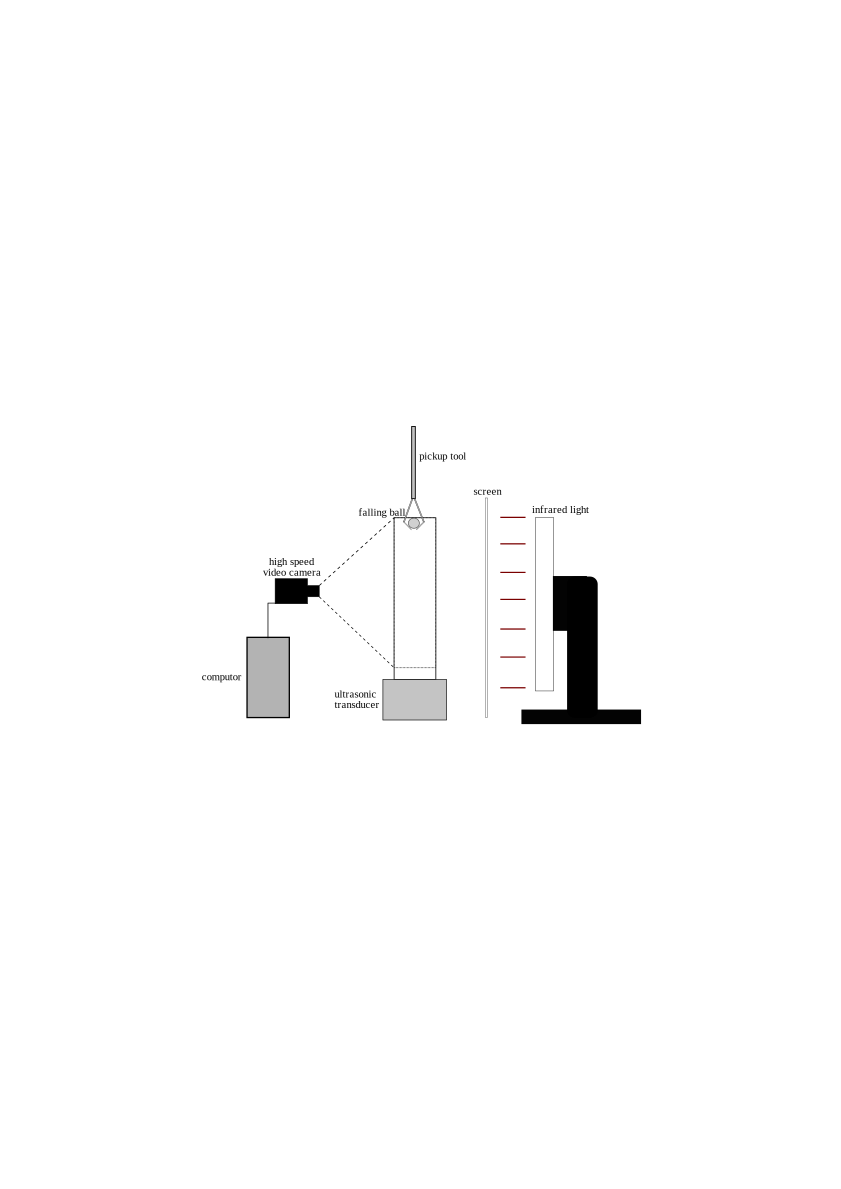
\includegraphics[clip,width=12.0cm]{X-Appendix/device.png}
    \caption{Schematic view of the experimental apparatus.}
    \label{fig:device2}
\end{figure}

\subsection{落下球 実験結果}

1wt.\%PAA溶液中における球の落下速度を解析した結果をFig.\ref{fig:1-1PAA-falling}に示す.縦軸は落下速度,横軸は落下開始時からの経過時間である.先述の電磁石ホルダを用いたFig.\ref{fig:1PAA-falling}とは異なり,超音波照射の有無において落下速度の高速化は見られなかった.一方で,先行研究であるIwamuro {\it et al.}\cite{ref:9}と同様に初めの加速後は減速し一定速度となった.

また,電磁石ホルダを用いた場合と同様に,超音波照射なしの状態における1から5試行目の結果をFig.\ref{fig:1-1PAA-falling1-5}に,6から10試行目の結果をFig.\ref{fig:1-1PAA-falling6-10}に示す.また,超音波照射ありの状態における1から5試行目の結果をFig.\ref{fig:1-1onPAA-falling1-5}に,6から10試行目の結果をFig.\ref{fig:1-1onPAA-falling6-10}に示す.これら試行ごとの結果において,先述のFig.\ref{fig:1PAA-falling1-5}-\ref{fig:1onPAA-falling6-10}の結果とは異なり落下速度のばらつきが非常に小さくなっていた.

\begin{figure}[ht]
    \centering
    \includegraphics[width=12cm,clip]{./X-Appendix/s1.png}
    \caption{Falling velocity of a sphere in 1wt.\%PAA solution with and without ultrasound irradiation.}
    \label{fig:1-1PAA-falling}
    \centering
    \includegraphics[width=12cm,clip]{X-Appendix/s1-0-1-5.png}
    \caption{Falling velocity of the sphere for each trial (\#1 to \#5) in 1wt.\%PAA solution without ultrasonic irradiation.}
    \label{fig:1-1PAA-falling1-5}
\end{figure}
\begin{figure}[ht]
    \centering
    \includegraphics[width=12cm,clip]{X-Appendix/s1-0-6-10.png}
    \caption{Falling velocity of the sphere for each trial (\#6 to \#10) in 1wt.\%PAA solution without ultrasonic irradiation.}
    \label{fig:1-1PAA-falling6-10}
    \centering
    \includegraphics[width=12cm,clip]{X-Appendix/s1-39-1-5.png}
    \caption{Falling velocity of the sphere for each trial (\#1 to \#5) in 1wt.\%PAA solution with ultrasonic irradiation.}
    \label{fig:1-1onPAA-falling1-5}
    \centering
    \includegraphics[width=12cm,clip]{X-Appendix/s1-39-6-10.png}
    \caption{Falling velocity of the sphere for each trial (\#6 to \#10) in 1wt.\%PAA solution with ultrasonic irradiation.}
    \label{fig:1-1onPAA-falling6-10}
\end{figure}

\subsection{考察}

電磁石ホルダを用いた把持方法と爪式ピッキングツールを用いた把持方法では試行ごとの落下速度の時間変化や超音波照射による高速化の有無において変化が見られた.以下に把持方法の変化による影響に関して検討を行う.

まず,電磁石ホルダを使用する場合,落下開始1分前に電源を切り,電磁石ホルダの把持力をゼロにする.しかし,落下させる対象の鋼球や溶液中に把持しているために存在する鋼製棒に磁性が残っている.また,落下球はPAA溶液中に存在するため浮力や粘弾性の影響を受ける.そのため落下開始時まで,把持している鋼製棒に接触したままとなっている.ここに,非常に弱い撃力を指で与え,落下させている.撃力による初速への影響
弾性によって減速が大きくなる可能性が存在する.

続いて,ピッキングツールを使用する場合に関して検討を行う.ピッキングホルダは球の把持を行っている爪を開くことによって,落下球の把持を開放し,球が落下する.爪を開放し球が落下する際,爪に球が干渉し,球がわずかに回転しながら落下していることが見られることが多かった.回転によって,超音波照射を行ったことで落下球周囲へ形成された,音響境界層へ影響を及ぼした可能性が考えられる.

また,電磁石ホルダは水槽と同じサイズの容器で覆われているため,水平方向の落下位置は水槽中心である.加えて,鉛直方向は水槽上部に固定しているため一定である.一方でピッキングツールは,マグネットベースに接続されて固定されたクランプで把持した.しかし,クランプの機構的特性上,水平方向の落下位置が球の直径$D$=10mm分ずれることがあった.
このことにより,都度位置が完全に一致しないことで,試行ごと落下経路が異なり履歴効果があまり見られなかったのだと考えられる.また,中心精度が不十分であったため,超音波圧力場の影響が受けきれず高速化が見られなかったとも考えられる.

\end{appendices}
\end{document}